% LaTeX resume using res.cls
\documentclass[margin]{res}
\usepackage{helvetica} % uses helvetica postscript font (download helvetica.sty)
\usepackage{fontspec}
\usepackage{graphicx}
%\usepackage{geometry}

\setromanfont{STSong} % 可以添加系统字体
\setmonofont{Courier New} % 等寬字型

\newfontfamily\hei{Heiti SC Medium}
%\geometry{left=2cm, right=2cm, top=2cm, bottom=2cm}

%\usepackage{helvetica} % uses helvetica postscript font (download helvetica.sty)
%\usepackage{newcent}   % uses new century schoolbook postscript font 
\setlength{\textwidth}{5.1in} % set width of text portion

\begin{document}

% Center the name over the entire width of resume:
% Draw a horizontal line the whole width of resume:
 \moveleft\hoffset\vbox{\hrule width\resumewidth height 1pt}\smallskip
% address begins here
% Again, the address lines must be centered over entire width of resume:
 \moveleft.5\hoffset\centerline{张文个人求职简历}
 \moveleft.5\hoffset\centerline{\\}
 \moveleft.5\hoffset\centerline{电话:13260027332\qquad{邮箱:1091681793@qq.com}}

 % \name{张文\\[12pt]}     % the \\[12pt] adds a blank
				        % line after name      

                        
                                       
\begin{resume}
    \begin{minipage}[t]{0.8\textwidth}
        \section{\hei{求职意向}} {\hei{人工智能算法工程师(以NLP为主,语音图像也有相应项目经验)}}
        % \section{\hei{联系方式}}  {\hei{电话:13260027332; 邮箱: w1091681793@gmail.com}}
        \section{\hei{教育经历}} {\sl 硕士  } \qquad{北京邮电大学}\qquad{计算机科学与技术}   \hfill 2014/09-2017/03 \\
                              {\sl 学士   } \qquad{武汉轻工大学}\qquad{网络工程}          \hfill 2010/09-2014/06 \\
        \section{\hei{获奖荣誉} }{入选2024年国家知识产权局青年拔尖人才(全局一共10人)} \\
                                {入选2023年国家知识产权局第七批骨干人才} \\
                                {2022和2023年连续两年信息中心年度优秀员工称号}
                                 

        \end{minipage}
            \hfill 
            \begin{minipage}[t]{0.1\textwidth}
                \begin{center}
                    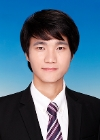
\includegraphics[width=60pt, height=80pt]{./suit.jpg}
                \end{center}
            \end{minipage}


\section{\hei{专业技能} }
            {\hei {语言及框架:}} 熟练掌握Python, C++, Java、JS等语言, 熟练掌握基于pytorch,tensorflow, deepspeed等深度学习开发框架,oat++、flask等后端服务框架,以及reactJS的前端开发框架。 \\
            {\hei {相关技术:}} . 熟练掌握LLM、Transformer, BERT,GPT等多种深度学习模型,在业务拓展和研究中,\\有一定的模型运用和创新基础和经验, 能够及时掌握和追踪AI相关技术发展。\\

\section{\hei{项目工作经历}} 
                {\hei{中国专利信息中心 } }  \hfill 2021.04-至今
                \begin{itemize}  \itemsep -2pt %reduce space between items
                \item[a.] 基于BERT、CNN等模型开发发明专利IPC智能辅助分类模型。
                \item[b.] 基于whisper、torchscript、sherpa-onnx、tritonserver等技术进行中文语音转文字的系统搭建。
                \item[c.] 基于fairseq以及ctranslate2等技术开发多语言机器翻译(主要涉及中到日、中到韩以及中到德)。
                \item[d.] 基于ReactJS、oat++等技术开发多语言翻译系统自主开发以及价值评估系统开发。
                 
                \end{itemize}
                {\hei{CLASSIII株式会社 } }  \hfill 2019.11-2021.03
                 \begin{itemize}  \itemsep -2pt %reduce space between items
                 \item[a.] 基于pytorch自研transformer等模型开发多语言短文本翻译模型(日到东南亚小语种)。
                \item[b.]  基于fairseq、flask等技术开发日英双语互译模型及服务,其中日英模型精度超过业界\\最好的模型deepL.
                \item[c.] 基于fairseq、flask等技术开发小样本训练样集翻译模型及服务,在保证模型通用泛化能力\\的同时,增加个性化领域的翻译能力。
                
                \end{itemize}
 
                {\hei{京东世纪贸易公司}} \hfill 2018.01-2019.10 \\
                 \begin{itemize}  \itemsep -2pt %reduce space between items
                    \item[a.] 基于tensorflow自研的DNN、DCN等模型开发京东APP首页广告位电商广告推荐精排模型,\\完成『千人千面』广告推荐。
                    \item[b.] 基于tensorflow、k8s等技术开发深度学习分布式训练框架,\\以满足内部广告部门使用。
                 %\item 网址:http://siyuanlib.com
                 \end{itemize} 

                {\hei{北京尚德机构}} \hfill 2017.04-2017.12 \\
                \begin{itemize}
                    \item[a.] 基于xgboost等模型开发舆情系统。针对尚德机构赏论坛中学员与老师的对话,对学员或\\老师的话术进行正向、中向以及负向的三分类分析,以提前定位并解决教学过程中的问题,\\同时提升教学服务质量。
                    \item[b.] 基于xgboost、tensorflow自研的cnnText、LSTM等模型开发主观题自动评分系统。 针对尚德机构老师对学员试卷问卷时效过长的问题,以人工智能算法为基础,\\开发相应主观题自动评分系统,以提升工作效率。
                \end{itemize} 


\end{resume}
\end{document}




